\section{Power and sample size for logistic regression} \label{sec:logistic-power}

The goal of many studies is to determine if a given predictor $X$ has
an effect on a binary outcome variable.
In planning such studies it is often crucial to determine the sample
size required in order to have a reasonable chance to detect an effect
of a given size.  Alternatively, if a study failed to detect a significant
effect, we might wish to determine if no real effect is present, or if
the sample size in the study was just insufficient to detect it.

In either case, power and sample size determination requires that we specify the Type I error rate, $\alpha$, of the test, and the \glossterm{effect size}
we wish to detect.  In the simple logistic model with one predictor,
\begin{equation*}
 \log \frac{\pi}{1-\pi} = \beta_0 + \beta_1 X
 \comma
\end{equation*}
the null hypothesis is $H_0 : \beta_1 = 0$, and the size of the effect
depends directly on the magnitude of the slope $\beta_1$.
That is, power increases with $| \beta_1 |$;  correspondingly, the sample
size required to detect an effect of given size (i.e., reject $H_0$ at
a given $\alpha$-level)
decreases with $| \beta_1 |$.

The difficulty in practice is that it is often difficult for the
researcher to specify the size of meaningful effect in terms of the
slope $\beta_1$ of the logistic model.
We describe below two standard situations in which effect size of interest
may be specified more simply to determine approximate power or
required sample size.

\subsection{Binary predictor: Comparing two proportions}
When there is a single binary predictor (and a binary response),
we may take $X=0$ for Group 1, and $X=1$ for Group 2,
so that $\beta_1$ is the log odds of ``success'' response in Group 2
as compared to Group 1.  

But, in this case
the data comprise a $2\times 2$ table, and the test of the logistic model
is analogous to a test of the difference of proportions in
two independent samples.  That is, $H_0 : \beta_1 = 0$ is
analogous to the test of $H_0 : \pi_1 = \pi_2$.
In this case the sample difference, $p_1 - p_1$
has an approximate large-sample normal distribution, with variance
\begin{equation*}
 \sigma_{p_1 - p_2}^2 = \frac{\pi_1 (1 - \pi_1)}{n_1} +
 \frac{\pi_2 (1 - \pi_2)}{n_2}
 \period
\end{equation*}

Assume that we are interested in being able to reject the null
hypothesis when the true difference  $|\pi_1 - \pi_2| = \pi_d$ is at least
some given value.  $\pi_1$ and $\pi_2$ (or $\pi_1$ and $\pi_d$)
provide a reasonable way to
specify the size of the effect of interest in this situation.

For example, in planning the arthritis treatment
experiment, the investigators might assume that
the probability of at least some improvement would be around $\pi_2 = 0.30$
with the placebo, and wish to have a high probability of rejecting
$H_0$ when the probability of at least some improvement with the active
treatment                                                                                                                                                     
is $\pi_1 = 0.50$
or greater.  The difference $\pi_d$ is usually the smallest difference
of substantive interest.  We also assume that $n_1 = n_2$.

Then the power of a two-tailed $\alpha$-level test of 
$H_0 : |\pi_1 - \pi_2 | = 0$
against the alternative $H_1: |\pi_1 - \pi_2| = \pi_d$
is approximately
\begin{eqnarray}
\mbox{power} & = & \Pr \left(
 \frac{ | p_1 - p_2 | - \pi_d }{ \sigma ( p_1 - p_2 ) }
 \right) \ge z_{1-\alpha/2} \nonumber \\
 & = & \Pr [ z > z_{1-\alpha /2} - \pi_d \, \sigma_{p_1 - p_2} ]
     + \Pr [ z < z_{\alpha /2} - \pi_d \, \sigma_{p_1 - p_2} ] \nonumber \\
 & = & 1- \Phi [z_{1-\alpha /2} - \pi_d \, \sigma_{p_1 - p_2}]
     + \Phi [z_{\alpha /2} - \pi_d \,  \sigma_{p_1 - p_2}] \label{eq:power2x2}
\end{eqnarray}
where $\Phi(\bullet)$ is the cumulative normal probability calculated by the
\FUNC{probnorm}.  For example, with $\alpha=0.05$, $\pi_1=0.30$,
and $\pi_2=0.50$, and a sample size of $n = n_1 + n_2 =80$, \eqref{eq:power2x2}
gives power = 0.462 when $\pi_2 = 0.50$ ($\pi_d = 0.20$)
and power =  0.807 when $\pi_2 = 0.60$ ($\pi_d = 0.30$).

It is often more convenient to find the sample size required for a
given power.  Using $\beta = 1- \mbox{power}$ as the probability of
a Type II error,%
\footnote{Don't confuse $\beta = 1- \mbox{power}$ here with the slope, $\beta_1$,
and intercept, $\beta_0$ of the logistic regression model.  Both uses
are conventional, and there are only a limited number of Greek letters
to go around.}
the approximate sample size required may be calculated as
\begin{equation}\label{eq:nbinlog}
n_1 = n_2 = \frac{ (z_{1-\alpha /2} + z_\beta) ^2 [ \pi_1 (1-\pi_1) + \pi_2 (1-\pi_2) ]} { (\pi_1 - \pi_2)^2 }
\end{equation}

These calculations (\eqref{eq:power2x2} and
\eqref{eq:nbinlog}),
along with tabular and graphical displays of power vs.\ $n$, are performed by the \macro{POWER2X2},
described in \macref{mac:power2x2}.
The tabular display is more useful for finding the exact calculated value,
while the graphs, as usual, show the overall behavior better.

\begin{Example}[arthrit13]{Arthritis treatment}
For the arthritis treatment data, we can perform a power analysis
for $\pi_1 = 0.30$ and $\pi_d = 0.2 \,(0.1)\, 0.4$ with the following
statement:
\begin{listing}
%power2x2(p1=.30, diff=.2 to .4 by .1, plot=power * n=diff);
\end{listing}
By default, the program calculates power for a range of sample sizes,
typically 10--200, though any range may be specified with the
\mparm{NMIN}{POWER2X2} and the \mparm{NMAX}{POWER2X2}.

In addition to printed output (not shown), the macro produces a 
graph of power against total sample size ($n = n_1 + n_2$)
shown in \figref{fig:power2x2a}.
For a desired power of $1-\beta$ = 0.80, the required total
sample size is about 80--85 when $\pi_d = 0.3$, but only
about 45--50 when $\pi_d = 0.3$.
In the data, $p_1 = 28/41 = 0.683$ and $p_2 = 14/43 = 0.325$,
so with $n=83$ there was adequate power.
%% one figure
\begin{figure}[htb]
  \centering
  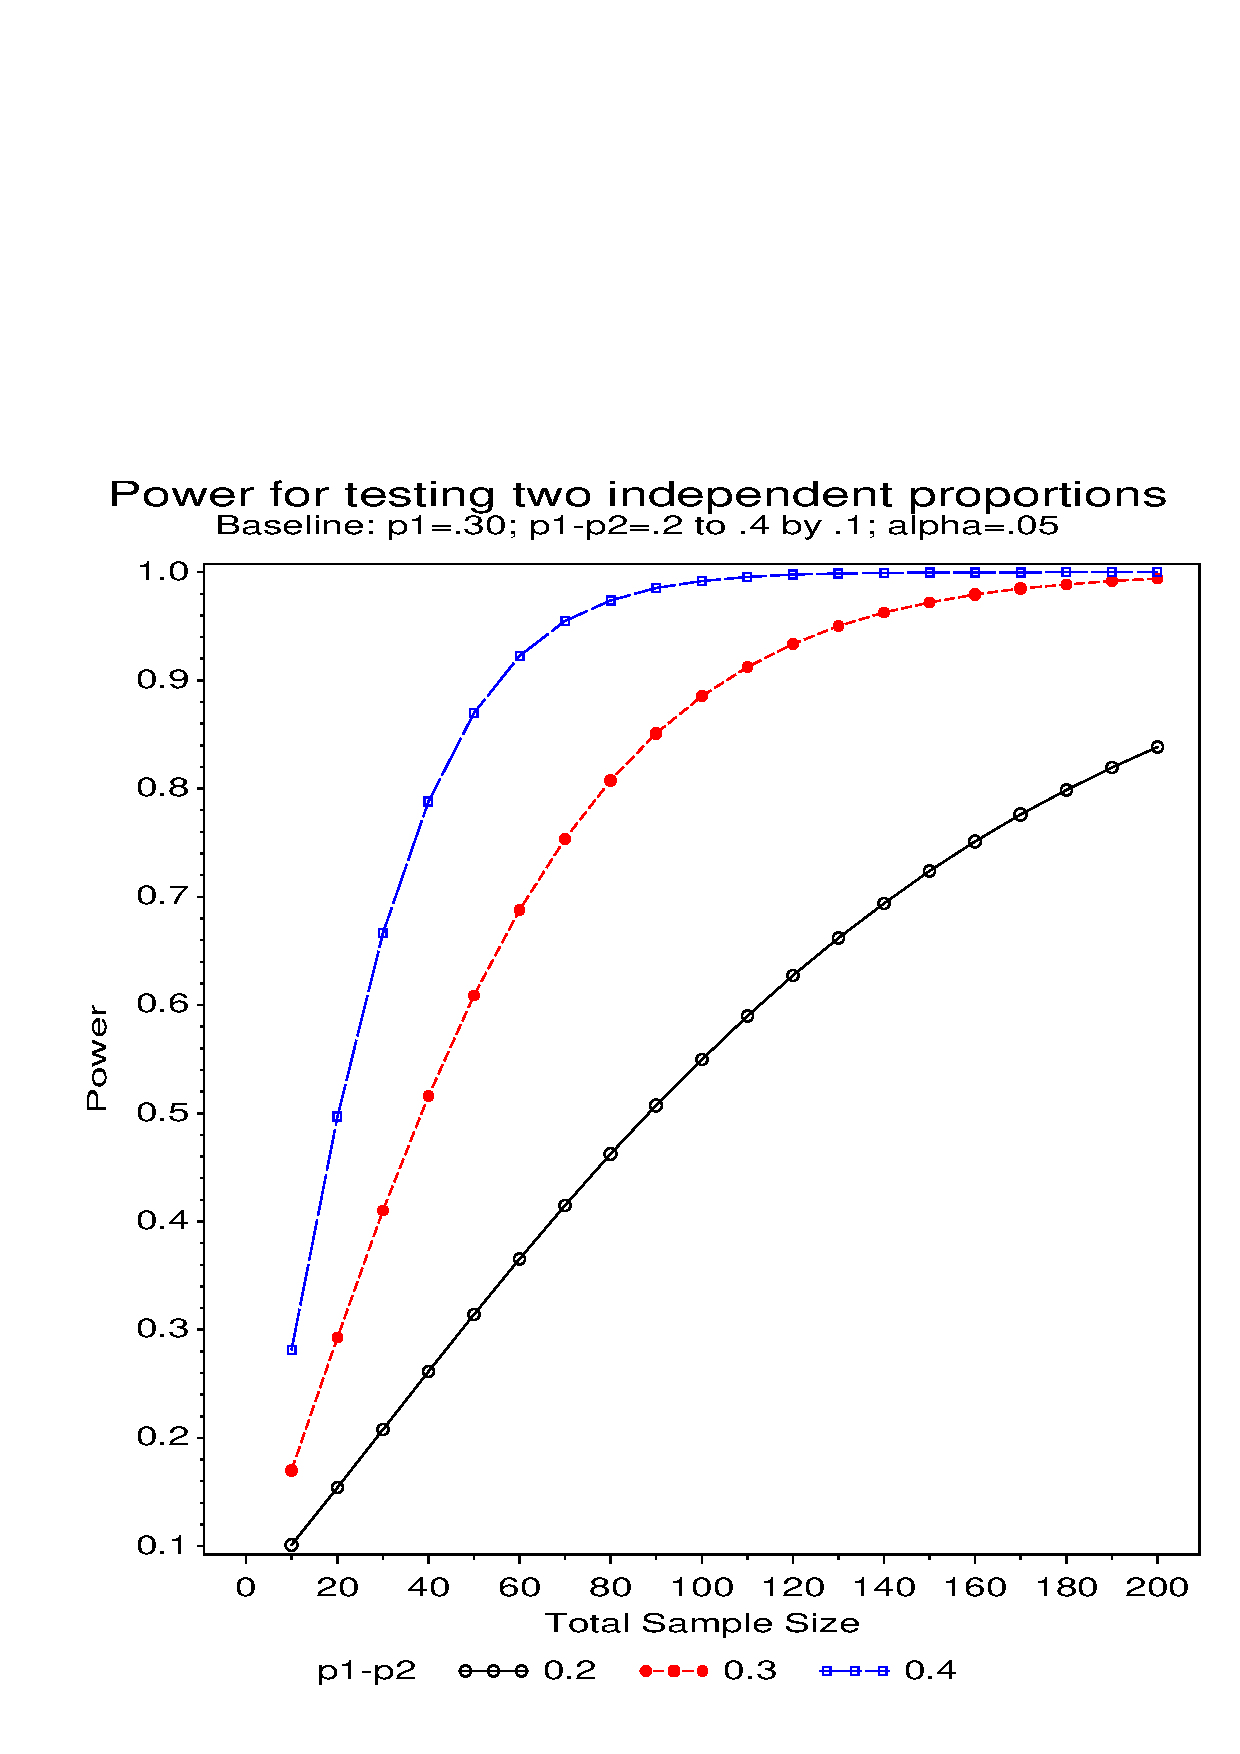
\includegraphics[scale=.6]{ch6/fig/power2x2a}
  \caption{Power analysis for arthritis treatment data}%
  \label{fig:power2x2a}
\end{figure}
\end{Example}

\subsection{Quantitative predictor}
When the predictor is quantitative, 
a simple method to specify the size of the
effect of interest is given by \citet[p. 131]{Agresti:96}
based on \citet{Hsieh:89}.
The slope $\beta_1$ under an alternative hypothesis
may be given in terms of the probabilities, $\pi_1$
and $\pi_2$ at two points, corresponding to
$X = \bar{X}$ and $X = \bar{X} + 1\mbox{s.d.}$
From these values, the effect size
can be specified in terms of the the odds ratio, 
$\theta = (p_2/(1-p_2)) \div (p_1/(1-p_1))$.

Letting $\psi = \log ( \theta )$,  Hseih provides the following
formula for the approximate sample size, $n$ required for a
one-tailed test with Type I error rate $\alpha$ and power $=1-\beta$:
\begin{equation}\label{eq:powerlog}
n = \frac{[z_{\alpha} + z_{\beta} \exp( -\psi^2 /4) ]^2 (1 + 2 p_1 \delta )} { p_1 \psi^2}
\end{equation}
where 
\begin{equation*}
\delta = \frac{1 + (1 + \psi^2) \exp( 5 \psi^2 /4) } {1 + \exp( -\psi^2 /4) }
\end{equation*}

In multiple logistic regression, larger sample sizes are required to
detect the \emph{partial} effect of one variable to the extent that
this variable is correlated with other explanatory variables
(because holding the other variables fixed then removes some of the
effect of the variable of interest).
If $R^2$ is the squared multiple correlation of the target predictor
with other predictors in the model, the unique variance of the
target variable is $1-R^2$.
To use formula \eqref{eq:powerlog} in this situation, let
$p_1$ refer to the probability of the event at the mean level of all
predictors, and divide the result of \eqref{eq:powerlog}
by $1-R^2$.
A more comprehensive approach to power analysis for 
logistic regression with multiple
covariates is described by \citet{Whittemore:81}.

These calculations are carried out by the \macro{POWERLOG},
described in \macref{mac:powerlog}.
The values of the input parameters
\pname{P1}, \pname{P2}, \pname{ALPHA}, \pname{POWER}, and \pname{RSQ},
may be supplied as macro arguments, or as variable values in an
input \Dset.
Output includes both a table and a graphical display.
\begin{Example}[power1]{Power for one or more predictors}
The following statement calculates the power of a test for $X_1$
when the probability of the event at $X = \bar{X}$ is $p_1 = 0.50$
and the probability of the event is expected to increase to
$p_1 = 0.75$ when $X$ increases to $X = \bar{X} + 1\mbox{s.d.}$.
By default, the macro calculates power for values of $R^2 = 0 (0.2) 0.6$.

\begin{listing}
%powerlog(p1=.5, p2=.75);
\end{listing}

The printed output is shown in \outref{out:powerlog.1}.
By default, the program uses the \pname{PLOT} statement,
\pname{PLOT N * POWER=RSQ}, producing the graph
in \figref{fig:powerlog}.
For a given power, the sample size to detect the effect of $X_1$ is smallest when $X_1$ is uncorrelated with other predictors.
For a given effect size, the sample size is also smallest when
$p_1 = 0.50$, as in this example.
\begin{Output}[htb]
\caption{Power table from \macro{POWERLOG}}\label{out:powerlog.1}
\small
\verbatiminput{ch6/out/powerlog.1}
\end{Output}

%% one figure
\begin{figure}[htb]
  \centering
  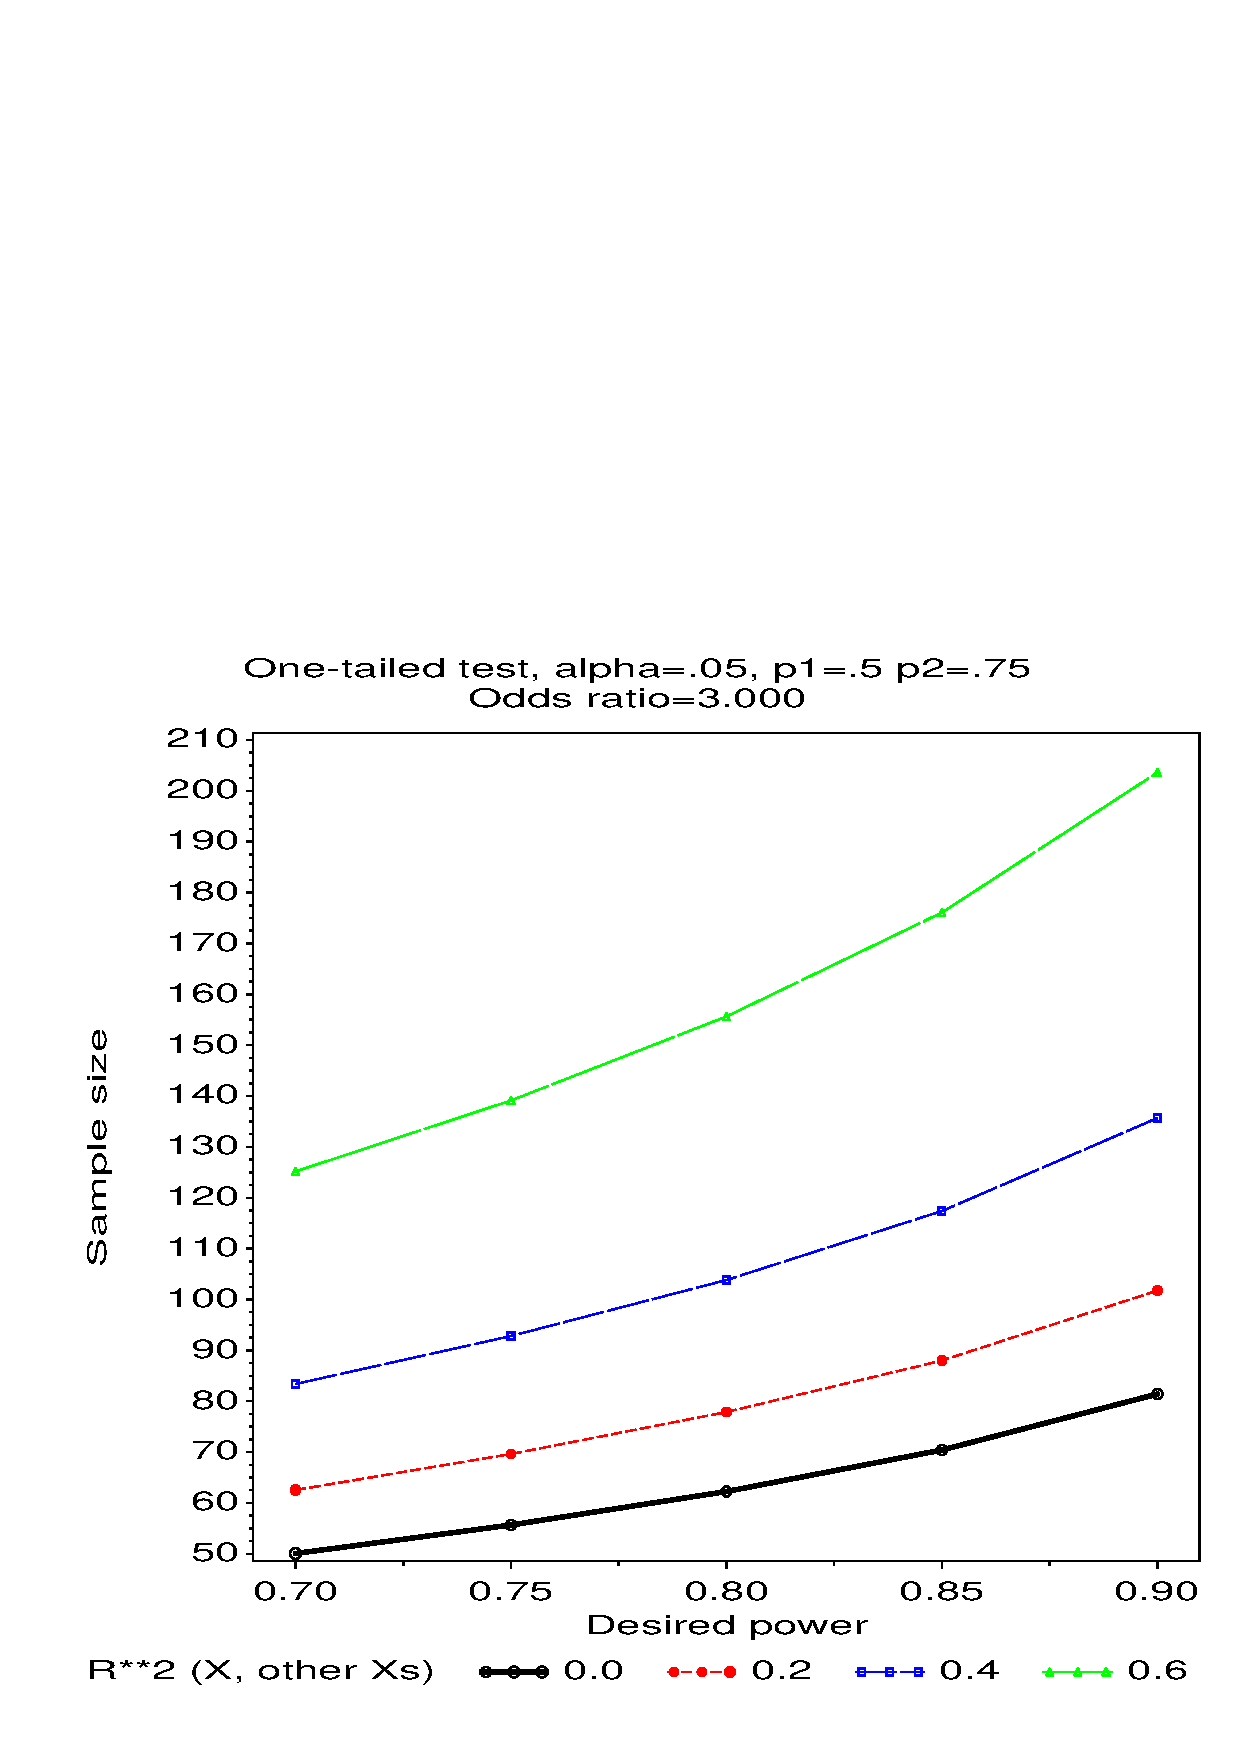
\includegraphics[scale=.6,clip]{ch6/fig/powerlog}
  \caption{Sample size display from \macro{POWERLOG}}%
  \label{fig:powerlog}
\end{figure}
\end{Example}

